%-- Intro --%

\begin{tframe}{Introduction}

\vspace{0.5cm}
Digital images are easy to manipulate thanks to the availability of the \textbf{powerful editing software} and \textbf{sophisticated digital cameras}.

\vspace{1cm}


\begin{minipage}{\textwidth}
\begin{columns}[T]
\begin{column}{0.5\textwidth}
\vspace{0.1cm}
The development of methods for verifying \textbf{image authenticity} is a real need in forensics.

\vspace{0.8cm}
\textbf{Purpose}: to detect image splicing  aimed at \emph{deceiving} the viewer.
\end{column}
\begin{column}{0.4\textwidth}

\includegraphics[width=0.8\textwidth]{images/image-editing.jpg}
\end{column}
\end{columns}
\end{minipage}

\end{tframe}

%-- Image compositions --%

\begin{tframe}{Forgery detection}
\vspace{0.2cm}
Image splicing detection techniques are based on \textit{inconsistencies}:
\vspace{0.3cm}
\begin{enumerate}
\item \textbf{Image resampling, copy-paste}: deduced from image metadata.
\vspace{0.3cm}

\item \textbf{Compression-based inconsistencies}: JPEG compression introduces blocking artifacts. Manufacturers of digital cameras and image processing software typically use different JPEG quantization tables.
\vspace{0.3cm}

\item  \textbf{Neighboring pixels relationship inconsistencies}: when an image is spliced some artifacts can be created.
\vspace{0.3cm}
\item \textbf{Intrinsic image properties inconsistencies}: e.g. scene lights, shadows or perspective.
\end{enumerate}

\end{tframe}

%-- Light based detection --%

\begin{tframe}{Lighting-based inconsistencies}
\vspace{0.2cm}
Methods based on \textbf{lighting inconsistencies} are particularly \emph{robust}: a perfect illumination adjustment in a image composition is very hard to achieve.
\vspace{0.3cm}
\begin{center}
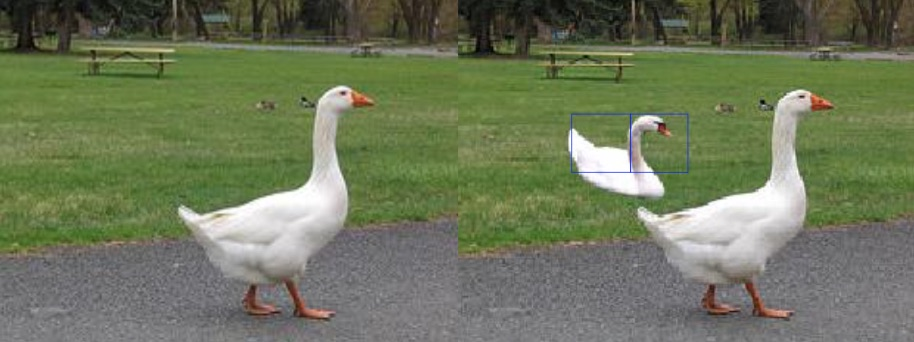
\includegraphics[width=0.5\textwidth]{images/ducks.jpg}
\vspace{0.1cm}
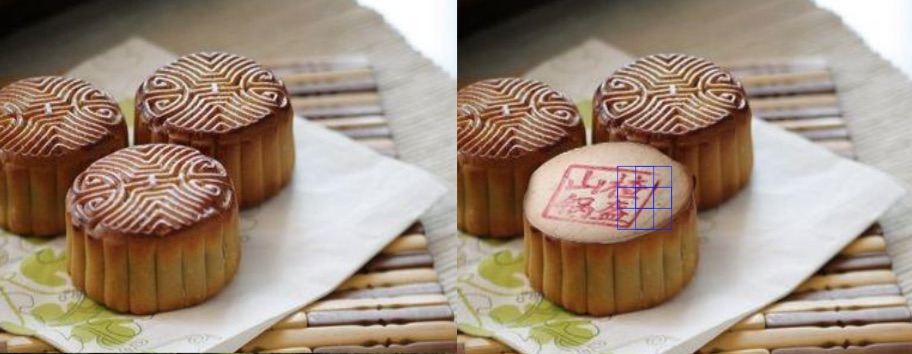
\includegraphics[width=0.5\textwidth]{images/cakes.jpg}
\end{center}
\end{tframe}

\begin{tframe}{Lighting-based inconsistencies}
\vspace{0.1cm}
These methods can be divided into two types of approaches:
\vspace{0.2cm}
\begin{enumerate}
\item \textbf{Object light source inconsistencies}: detected using \emph{shadows}, \emph{face geometry}, \emph{generic object surfaces}.
\vspace{0.2cm}

\item \textbf{Illuminant colors inconsistencies}: {\small assuming that a scene is lit by the same light source, all objects must have the same illuminant colors.}
\vspace{0.2cm}
\begin{enumerate}
\item \textit{Specular dichromatic reflectance models}
\vspace{0.1cm}
\item \textit{Illuminant Maps (IMs)}
\end{enumerate}
\end{enumerate}
\begin{center}
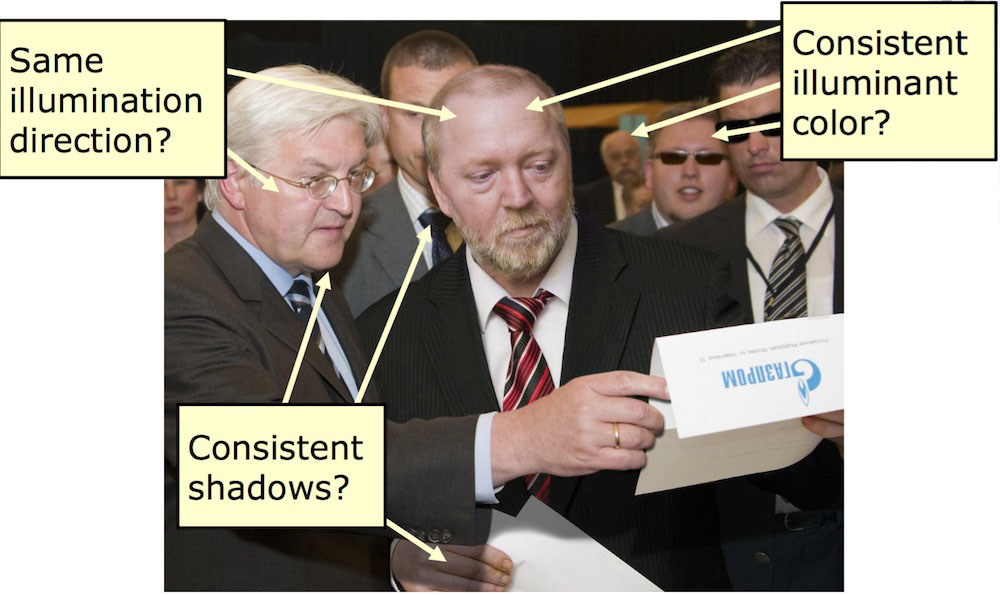
\includegraphics[width=0.4\textwidth]{images/lighting-based.jpg}
\end{center}
\end{tframe}

\begin{tframe}{Spectral dichromatic reflectance models\\{\small [Gholap and Bora 2008]}}
\vspace{0.1cm}
Reflection of any materials can be modelled as additive mixture of two components: \textbf{diffused reflection}. $L_B(\lambda)$, and \textbf{surface reflection}, $L_S(\lambda)$. So, the \emph{reflected light} can be written as:
$$L(\Theta, \lambda) = m_S(\Theta)* L_S(\lambda) + m_B(\Theta) * L_B(\lambda)$$

\begin{center}
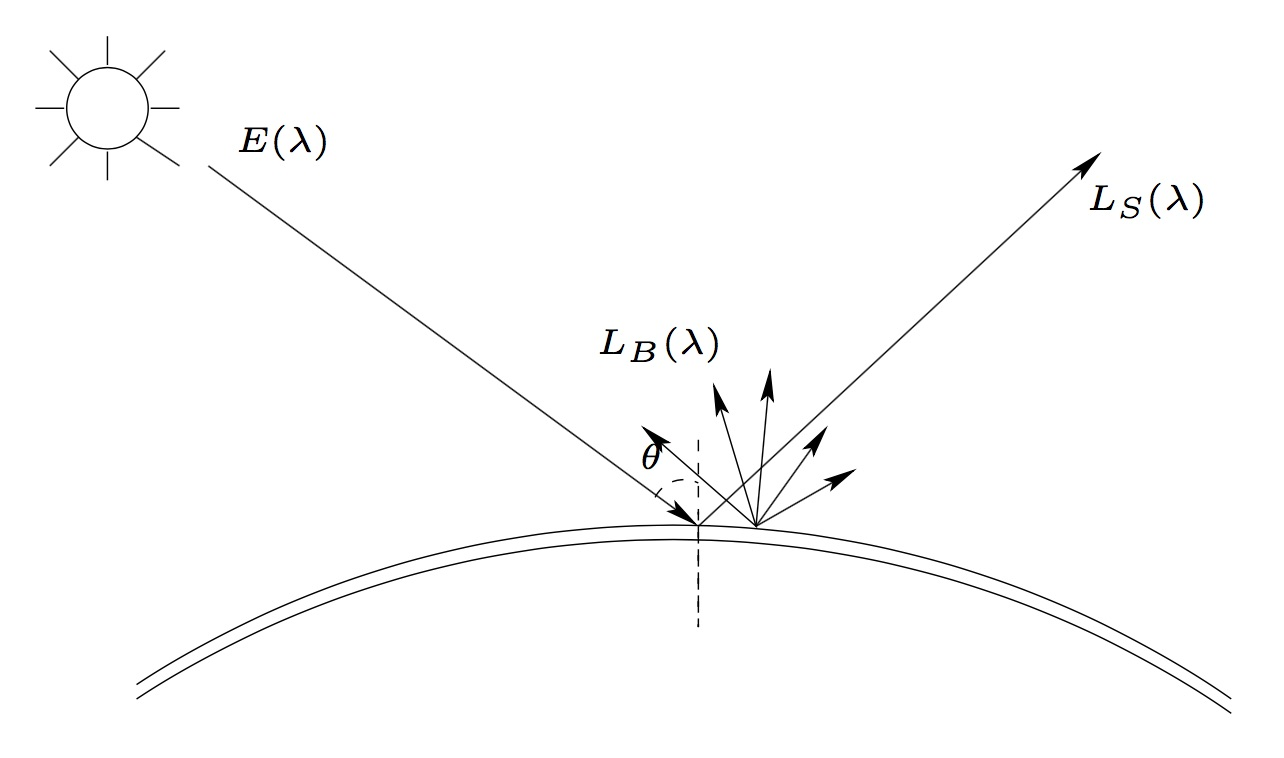
\includegraphics[width=0.4\textwidth]{images/reflectance.jpg}
\end{center}

The two vectors $L_B(\lambda)$ and $L_S(\lambda)$ span the two dimensional plane called \textbf{dichromatic plane}.
\end{tframe}


\begin{tframe}{Spectral dichromatic reflectance models\\{\small [Gholap and Bora 2008]}}
\vspace{0.1cm}
\begin{minipage}{\textwidth}
\begin{columns}[T]
\begin{column}{0.5\textwidth}
\vspace{0.4cm}
From the two \emph{dichromatic plane}, the \textbf{dichromatic line} is estimated: given two dichromatic lines of different objects, they intersects at a point giving the chromaticity values of the illuminant color. 

\vspace{1.1cm}

\textbf{Detection}: if a object is spliced into the image, ad error is introduced in the estimation.
\end{column}
\begin{column}{0.4\textwidth}
\centering
\vspace{1.5cm}

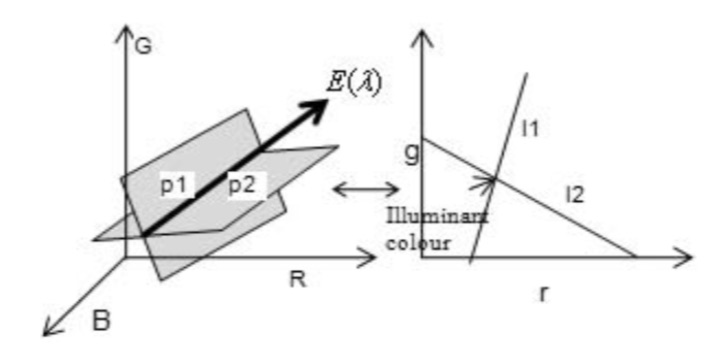
\includegraphics[width=\textwidth]{images/dichromatic-plane.jpg}
\end{column}
\end{columns}
\end{minipage}
\end{tframe}


\begin{tframe}{Illuminant estimation / color constancy methods}
\vspace{0.1cm}
\textbf{\emph{Color constancy}}: create an image, where the object representation is independent of the illumination color.
Under some assumptions this is equivalent to estimating the illuminant color.
\vspace{0.3cm}
\begin{small}
\begin{itemize}
\item \textbf{Gray world, maxRGB}: statistical-based
\vspace{0.1cm}
\item \textbf{Gamut mapping}: statistical-based
\vspace{0.1cm}
\item \textbf{Gray edge-* methods}: statistical
\vspace{0.1cm}
\item \textbf{Color by correlation}: physics-based
\vspace{0.1cm}
\item \textbf{Inverse-Intensity Chromaticity} (IIC): physics-based
\end{itemize}
\end{small}
\end{tframe}

\begin{tframe}{Illuminant Maps {\small [Riess and Angelopuolou 2010]}}
\vspace{0.1cm}
\textbf{Illuminant Maps} locally describe the \emph{color of the illuminant} of a image.
\vspace{0.1cm}
\begin{enumerate}
\item Estimate illuminant colors locally (\emph{using IIC})
\item Create the \emph{illuminant map} 
\item User selects a region with estimates of the dominant illuminants
\item Create a \textbf{distance map} between each local block
\end{enumerate}
\vspace{0.1cm}
\centering
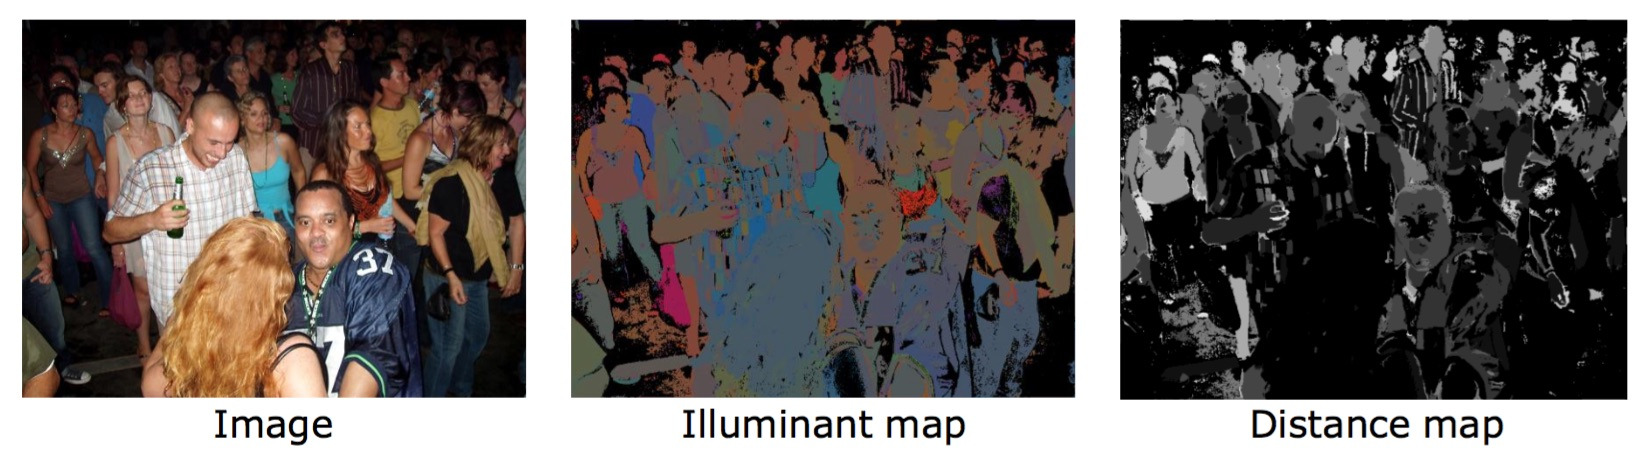
\includegraphics[width=\textwidth]{images/riess.jpg}
\end{tframe}

\begin{tframe}{Illuminant Maps {\small [Wu and Fang 2011]}}
The image is divided into overlapping blocks in order to estimate local illuminant colors.
\vspace{0.2cm}
\begin{enumerate}
\item Estimate illuminant colors locally (\emph{using Gray-World, Gray-Edge and Gray-Shadow})
\vspace{0.1cm}

\item Selecting best representation for each block using a \emph{maximum likelihood classifier}
\vspace{0.1cm}

\item Some blocks are selected as \textbf{references}
\vspace{0.1cm}

\item Evaluate the \textbf{angular error} between suspicious block and the reference blocks: if the distance exceeds a \emph{threshold}, the block is classified as spliced.
\end{enumerate}
\vspace{0.1cm}
\end{tframe}

\begin{tframe}{Illuminant Maps {\small [Carvalho \emph{et al.} 2013]}}
\vspace{0.1cm}
Tailored for image of \emph{human faces}. Requires user interaction in the face definition step.
\vspace{0.4cm}
\begin{center}
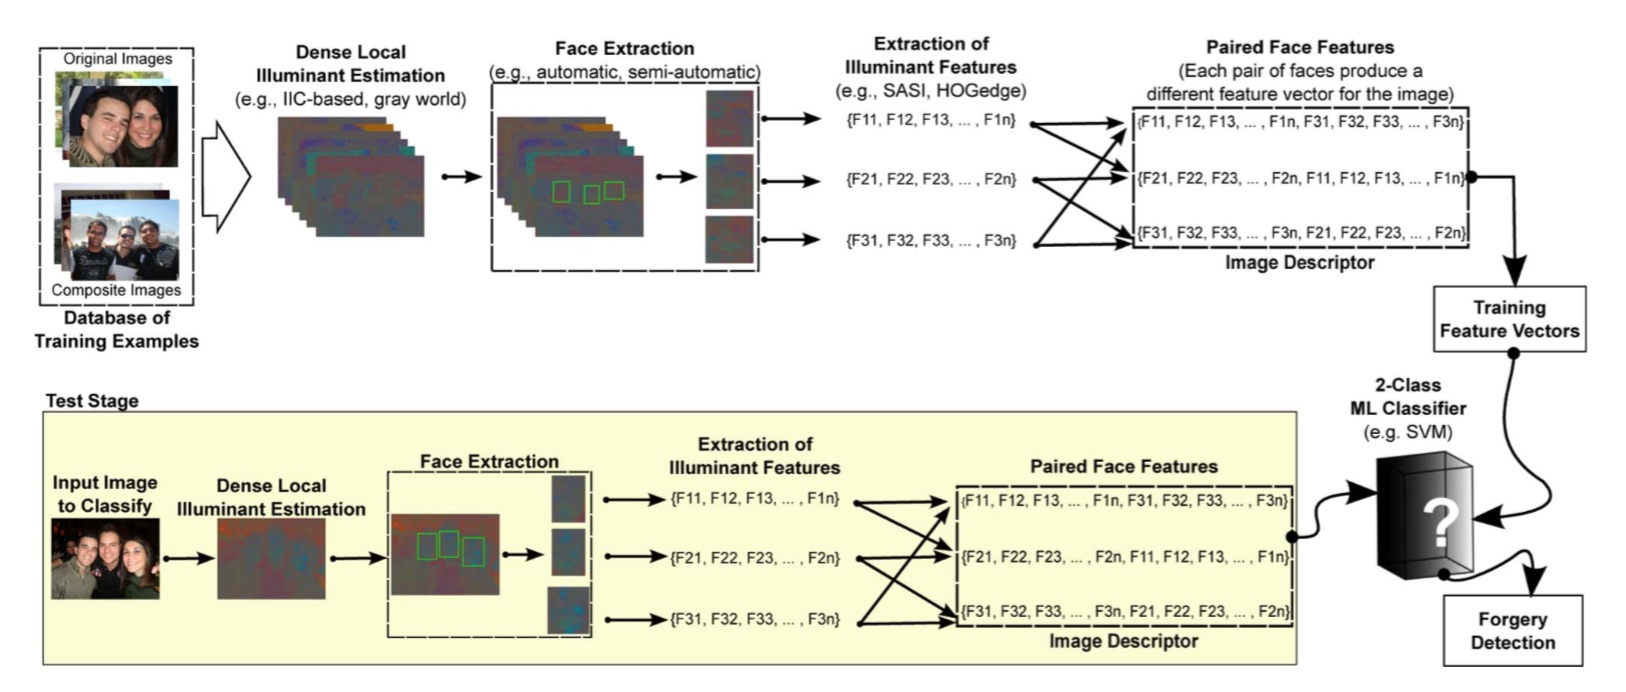
\includegraphics[width=\textwidth]{images/carvalho.jpg}
\end{center}
\end{tframe}

\begin{tframe}{Illuminant Maps {\small [Carvalho \emph{et al.} 2016]}}
\vspace{0.1cm}
Use the \textbf{statistical differences} between pristine and edited images through specific image descriptor.\vspace{0.4cm}
\begin{center}
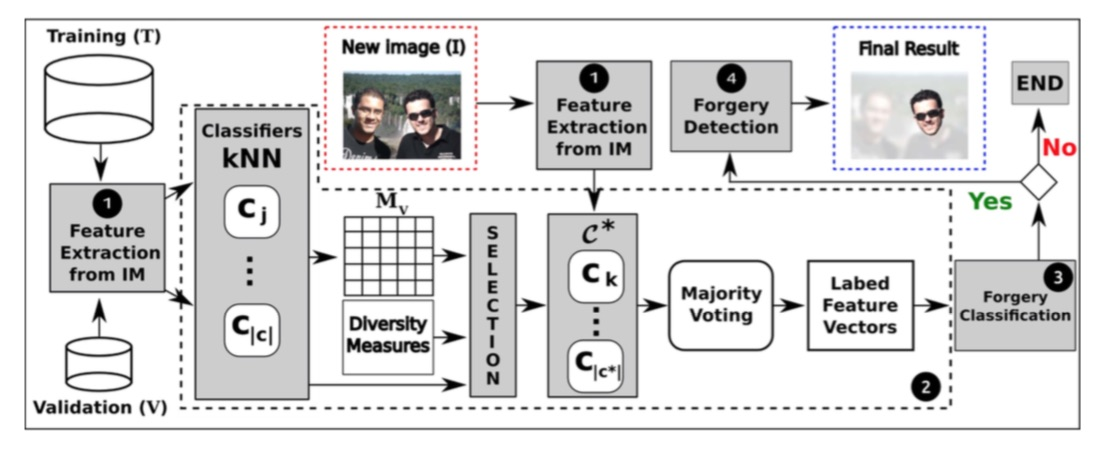
\includegraphics[width=\textwidth]{images/carvalho2.jpg}
\end{center}
\end{tframe}

\begin{tframe}{Illuminant Maps {\small [Schetinger \emph{et al.} 2016]}}
\vspace{0.1cm}
Extending previous work using different ways to use \textbf{combinations of different IMs}. It works on single ROIs.
\vspace{0.2cm}
\begin{minipage}{\textwidth}
\begin{columns}[T]
\begin{column}{0.5\textwidth}
\vspace{0.4cm}
\begin{small}
\begin{enumerate}
\item IM estimation using CGE and IIC
\item \textbf{Statistical difference}:
$$\vartheta = \frac{1}{q} \sum_{i = 1}^{q} \log (\| \lambda_i*(g_{GCE})^2 - \lambda_i*(f_{IIC})^2 \|)$$
\item Create \textbf{image descriptor} combining multiple eigenvalues
\item SVM classifier
\end{enumerate}

\end{small}
\end{column}
\begin{column}{0.4\textwidth}
\centering
\vspace{1.5cm}

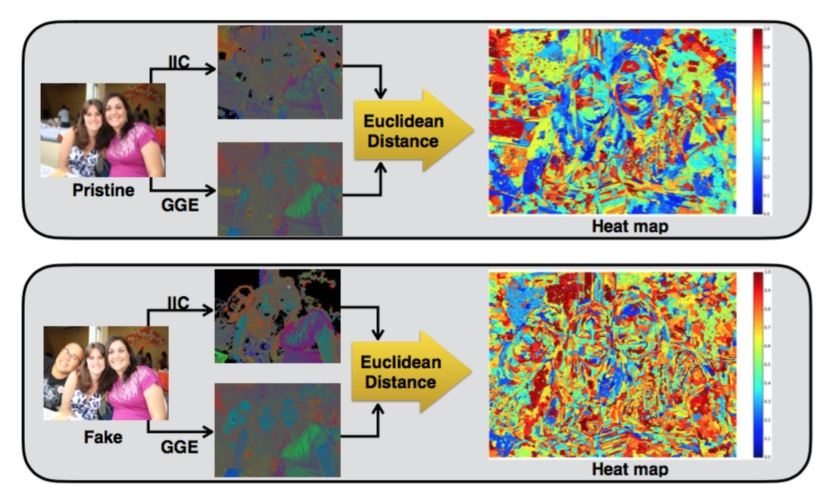
\includegraphics[width=\textwidth]{images/victor.jpg}
\end{column}
\end{columns}
\end{minipage}

\end{tframe}


